\documentclass[12pt]{article}

% Adjusted page margins to reduce vertical space
\usepackage[top=0.6in, bottom=1in,left=1in, right=1.2in]{geometry}

% Formatting and layout packages
\usepackage{titlesec}
\usepackage{lipsum}
\usepackage{mathpazo} % Font package for aesthetics

\usepackage{mdframed}

\newmdenv[
  topline=true, 
  bottomline=true,
  rightline=true, 
  leftline=true, 
  linecolor=black, 
  linewidth=0.8pt,
  backgroundcolor=white,
  innertopmargin=8pt,
  innerbottommargin=8pt,
  skipabove=8pt,
  skipbelow=8pt,
  splitbottomskip=2pt,  % Ensures proper spacing when the box splits across pages
  splittopskip=2pt,
]{solutionbox}

% Auto-wrap any "\item[Solution.]" in a solutionbox until next item at same level
\usepackage{xparse}
\usepackage{xstring}
\usepackage{etoolbox}

% Track nesting depth across list environments
\newcounter{solution@depth}
\newcounter{solution@level}
\newif\ifinsolutionbox
\insolutionboxfalse

% Increase/decrease depth for enumerate/itemize/description
\AtBeginEnvironment{enumerate}{\stepcounter{solution@depth}}
\AtEndEnvironment{enumerate}{%
  % If a solutionbox was opened at this level, close it before exiting
  \ifinsolutionbox
    \ifnum\value{solution@depth}=\value{solution@level}\relax
      \end{solutionbox}%
      \insolutionboxfalse
    \fi
  \fi
  \addtocounter{solution@depth}{-1}%
}
\AtBeginEnvironment{itemize}{\stepcounter{solution@depth}}
\AtEndEnvironment{itemize}{\addtocounter{solution@depth}{-1}}
\AtBeginEnvironment{description}{\stepcounter{solution@depth}}
\AtEndEnvironment{description}{\addtocounter{solution@depth}{-1}}

% Intercept \item to open/close solution boxes based on label
\let\olditem\item
\RenewDocumentCommand{\item}{o}{%
  % If we're starting a new item at the same level as an open solutionbox, close it
  \ifinsolutionbox
    \ifnum\value{solution@depth}=\value{solution@level}\relax
      \end{solutionbox}%
      \insolutionboxfalse
    \fi
  \fi
  % If no optional label, just pass through
  \IfNoValueTF{#1}{%
    \olditem
  }{%
    % If the label is exactly "Solution.", open a new solutionbox
    \IfStrEq{#1}{Solution.}{%
      \olditem[]%
      \begin{solutionbox}%
      \insolutionboxtrue
      \setcounter{solution@level}{\value{solution@depth}}%
    }{%
      \olditem[#1]% other labels unchanged
    }%
  }%
}



% Packages for figures and tables
\usepackage{graphicx}
\usepackage{subcaption}
\usepackage{svg}
\usepackage{booktabs}
\usepackage{float}

% Math-related packages
\usepackage{amsmath, amssymb, amsthm}

% TikZ for spacetime diagram
\usepackage{tikz}
\usetikzlibrary{arrows,arrows.meta,angles,quotes,calc}

% Declare supported graphic file types
\DeclareGraphicsExtensions{.pdf,.jpg,.tif,.png}

% Theorem and definition environments
\newtheorem{theorem}{Theorem}
\newtheorem{corollary}[theorem]{Corollary}
\newtheorem{lemma}[theorem]{Lemma}
\newtheorem{definition}{Definition}

% Reduce unnecessary vertical spacing
\setlength{\parskip}{0pt}  % No extra space between paragraphs
\setlength{\topsep}{2pt}   % Reduce spacing before lists/theorems
\setlength{\partopsep}{0pt}
\raggedbottom  % Prevents vertical stretching
\pagenumbering{gobble}

% Load hyperref last to apply hidelinks properly
\usepackage[hidelinks]{hyperref}

%%%%%%%%%%%%%%%%%%%%%%%%%%%%%%%%
\begin{document}
\thispagestyle{plain}
\vspace{-4ex}  % Less aggressive spacing reduction


\begin{center}
\begin{tabular}{*{3}{c}}
    \parbox[t]{0.3\linewidth}{\centering\textbf{Homework 2\\September 19, 2025}}
    & \parbox[t]{0.3\linewidth}{\centering\textbf{MATH 458\\General Relativity}}
    & \parbox[t]{0.3\linewidth}{\centering\textbf{Erise He}}\\[1em]
    \hline
\end{tabular}
\end{center}

\bigskip


\begin{enumerate}
  \item[Question 1] \textbf{More index manipulation practice.} Show that the "helpful identity" from HW 1, problem 5,
  \[
  (\Lambda^{-1})^{\alpha}{}_{\mu}\,\eta_{\alpha\nu} \,=\, \eta_{\mu\beta}\,\Lambda^{\beta}{}_{\nu}
  \]
  is true. You may find one of the "Useful Identities" from Chapter 4 to be useful as a starting point.
  
  \item[Solution.] 
    We start from eq. 4.18:
   $$\eta_{\alpha \beta}=\eta_{\mu \nu} \Lambda^\mu{ }_\alpha \Lambda^\nu{ }_\beta$$
   We multiply both sides of (4.18) by $\left(\Lambda^{-1}\right)^\alpha{ }_\mu$ and contract on $\alpha$ to get:
  
   $$\left(\Lambda^{-1}\right)^\alpha{ }_\mu \eta_{\alpha \beta}=\left(\Lambda^{-1}\right)^\alpha{ }_\mu\left(\eta_{\rho \sigma} \Lambda^\rho{ }_\alpha \Lambda^\sigma{ }_\beta\right)$$

   where i replaced $\mu, \nu$ by $\rho, \sigma$. Then we use the definition of the inverse metric to get:

   $$
  \begin{aligned}
  \left(\Lambda^{-1}\right)^\alpha{ }_\mu \eta_{\alpha \beta} & =\eta_{\rho \sigma} \underbrace{\left(\Lambda^{-1}\right)^\alpha{ }_\mu \Lambda^\rho{ }_\alpha}_{=\delta^\rho{ }_\mu} \Lambda^\sigma{ }_\beta \\
  & =\eta_{\rho \sigma} \delta^\rho{ }_\mu \Lambda^\sigma{ }_\beta\\
  & =\eta_{\mu \rho}  \Lambda^\sigma{ }_\beta
  \end{aligned}
  $$
  Then, if we simply rename the free indices, we get:

  $$\left(\Lambda^{-1}\right)^\alpha{ }_\mu \eta_{\alpha \nu}=\eta_{\mu \beta} \Lambda^\beta{ }_\nu$$


  \newpage





















  
  \item[Question 2] \textbf{Coordinate bases.} Book problem P5.2. (Most of problem 5.1 is either in box 5.1 or was done as an example in lecture. No need to re-do all of 5.1 here.)\\
  (Do problem P5.1 first.) Consider the coordinate basis discussed in box 5.1 for polar coordinates $r, \theta$.
    \item[(a)] We know that an object in uniform circular motion has a constant radius, so it must have a velocity $\boldsymbol{v}$ such that $v^r=0$. Use the polar-coordinate metric to show that if we assume this velocity has a constant (and coordinate-system-independent!) squared magnitude of $\boldsymbol{v} \cdot \boldsymbol{v}=v^2$, then we must have $v^\theta= \pm v / r$ (where the sign depends on which way the object moves around the circle).
    
    
    \item[Solution.]
    We write the velocity in polar coordinates:
    $$
    \mathbf{v}=v^r \mathbf{e}_r+v^\theta \mathbf{e}_t
    $$
    where $v^r=\frac{d r}{d t}$ , and $v^\theta=\frac{d \theta}{d t}$. From Box 5.1 the metric in $(r, \theta)$ is:
    $$
    g_{\mu \nu}=\left[\begin{array}{cc}
    1 & 0 \\
    0 & r^2
    \end{array}\right] \quad \Rightarrow \quad \mathbf{v} \cdot \mathbf{v}=g_{r r}\left(v^r\right)^2+2 g_{r \theta} v^r v^\theta+g_{\theta \theta}\left(v^\theta\right)^2=\left(v^r\right)^2+r^2\left(v^\theta\right)^2
    $$
    Since we know that $v^r=\dot{r}=0$, and if we assume the squared speed is constant ($\mathbf{v} \cdot \mathbf{v}=v^2$) and coordinate independent, then the above equation becomes:
    $$
    \begin{aligned}
    v^2 & =\left(v^r\right)^2+r^2\left(v^\theta\right)^2 \\
    & =r^2\left(v^\theta\right)^2
    \end{aligned}
    $$
    Thus, we have:
    $$
    v^\theta=\pm \frac{v}{r}
    $$
    where + for counter-clockwise motion and - for clockwise.
    
    \item[(b)] Find this object's velocity components $v^x$ and $v^y$ in cartesian coordinates. Express your result as a function of $r$ and $\theta$. Use a sketch to show that these components do indeed describe a vector tangent to a circle of radius $r$, and also show that the squared magnitude of this vector in the cartesian system is indeed $v^2$.
    
    \item[Solution.]
    
    
    we use the (contravariant) component transformation:
    $$
    A^\alpha=\frac{\partial x^\alpha}{\partial x^{\prime \mu}} A^{\prime \mu}
    $$
    where we denote $\left(x^\alpha\right)=(x, y),\left(x^{\prime \mu}\right)=(r, \theta)$. Then, since $x=r \cos \theta, y=r \sin \theta$, we have:
    $$
    J \equiv \frac{\partial(x, y)}{\partial(r, \theta)}=\left[\begin{array}{ll}
    \frac{\partial x}{\partial r} & \frac{\partial x}{\partial \theta} \\
    \frac{\partial y}{\partial r} & \frac{\partial y}{\partial \theta}
    \end{array}\right]=\left[\begin{array}{lr}
    \cos \theta & -r \sin \theta \\
    \sin \theta & r \cos \theta
    \end{array}\right]
    $$

    Since $v^r=0$, we get:
    $$
    \begin{aligned}
    v^x&=\frac{\partial x}{\partial r} v^r+\frac{\partial x}{\partial \theta} v^\theta=\cos \theta \cdot 0+(-r \sin \theta) v^\theta=-r \sin \theta v^\theta\\
    v^y&=\frac{\partial y}{\partial r} v^r+\frac{\partial y}{\partial \theta} v^\theta=\sin \theta \cdot 0+(r \cos \theta) v^\theta=r \cos \theta v^\theta
    \end{aligned}
    $$
    and then using the result from part (a), $v^\theta= \pm v / v$, we have:
    $$
    v^x=\mp v \sin \theta, \quad v^y= \pm v \cos \theta
    $$
    Finally, we check the squared magnitude in Cartesian coordinates
    $$
    \begin{aligned}
    \left(v^x\right)^2+\left(v^y\right)^2=v^2\left(\sin ^2 \theta+\cos ^2 \theta\right)=v^2
    \end{aligned}
    $$
    is indeed true.

    \begin{figure}[H]
    \centering
    \includegraphics[width=0.7\linewidth]{graph.png}
    \caption{vector tangent to a circle of radiu r}
    \end{figure}


    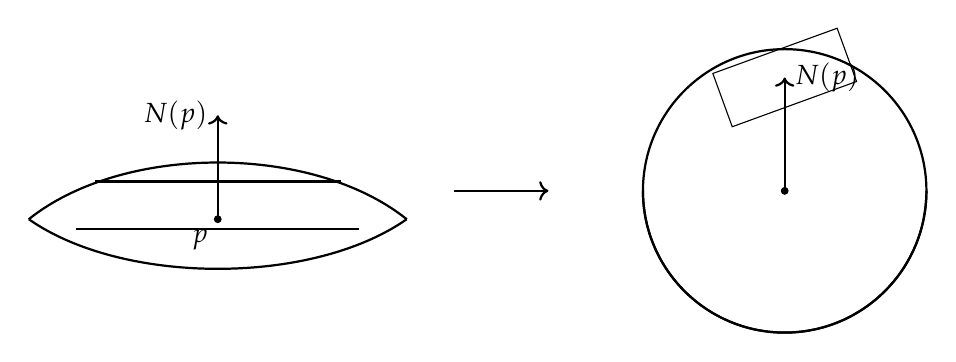
\begin{tikzpicture}[scale=1.2]
    
    % Left surface
    \draw[thick] (-2,-0.3) .. controls (-1,0.5) and (1,0.5) .. (2,-0.3);
    \draw[thick] (-2,-0.3) .. controls (-1,-1) and (1,-1) .. (2,-0.3);
    \draw[thick] (-1.5,-0.4) -- (1.5,-0.4);
    \draw[thick] (-1.3,0.1) -- (1.3,0.1);
    
    % Point p
    \filldraw (0,-0.3) circle (1pt) node[below left] {$p$};
    
    % Normal vector on surface
    \draw[->, thick] (0,-0.3) -- (0,0.8) node[left] {$N(p)$};
    
    % Arrow to right
    \draw[->, thick] (2.5,0) -- (3.5,0);
    
    % Right side: sphere
    \draw[thick] (6,0) circle (1.5);
    \draw[thick] (4.5,0) arc[start angle=180, end angle=360, radius=1.5];
    
    % Normal vector at sphere
    \filldraw (6,0) circle (1pt);
    \draw[->, thick] (6,0) -- (6,1.2) node[right] {$N(p)$};
    
    % Tangent plane as tilted square
    \draw[rotate around={20:(6,1.2)}] (5.3,0.9) rectangle (6.7,1.5);
    
    \end{tikzpicture}

    






  \newpage




















  \item[Question 3] \textbf{Metric on the surface of a sphere.}
  \item[(a)] \textbf{Book problem P5.6.} Consider polar-coordinate-like "radial-longitude" coordinates $r, \phi$ for the 2D surface of a sphere of radius $R$, where $r$ is the distance along the sphere's surface measured from the north pole and $\phi$ is an angular longitude coordinate measured around the pole. Note that curves of constant $r$ and curves of constant $\phi$ are always perpendicular to each other everywhere on the sphere. Therefore (as we did in Box 5.1 for polar coordinates), by considering displacements on the sphere's surface that lie purely in the $r$ and $\phi$ directions, infer the components $g_{\mu \nu}$ of the metric for this coordinate system (assuming we use a coordinate basis). Express these components purely in terms of $R$ and $r$. (We will later find a similar coordinate system helpful in describing the spatial geometry of the universe.)
  
  \item[Solution.] Given a 2D surface of a sphere of radius $R$, with coordinates $(r, \phi)$. Then, curves $r=$ const and $\phi=$ const are perpendicular everywhere, so the metric is diagonal in $(r, \phi)$ :
  $$
  d s^2=g_{r r}(r) d r^2+g_{\phi \phi}(r) d \phi^2
  $$
  where $g_{r \phi}=0$ because basis $\left\{\mathbf{e}_r, \mathbf{e}_\phi\right\}$ is orthogonal. Next, by definition of the arc length $r$ here, we should have:
  $$g_{r r}=1$$
  Then, at geodesic distance $r$, the corresponding colatitude is $\theta=\frac{r}{R}$, and the latitude circle has radius $R \sin \theta=R \sin \left(\frac{r}{R}\right)$. That is
  $$
  g_{\phi \phi}(r)=\left(R \sin \frac{r}{R}\right)^2
  $$
  together, we get:
  $$
  \begin{aligned}
  d s^2=d r^2+\left(R \sin \frac{r}{R}\right)^2 d \phi^2
  \end{aligned}
  $$
  where $g_{r r}=1$ and $g_{\phi \phi}=\left(R \sin \frac{r}{R}\right)^2$.



    \item[(b)] Let $r=\sin\theta$ and express the metric $g_{ij}$ in terms of $(r,\,\phi)$. Note this is a different definition of $r$ from the book problem, and the sphere here has $R=1$.
  
  \item[Solution.] Suppose we use the definition $r=\sin\theta$, then start from the usual spherical metric, 
  $$d s^2=d \theta^2+\sin ^2 \theta d \phi^2$$
  we define a new radial coordinate:
  $$r=\sin \theta \in[0,1]$$
  where $\theta=\arcsin r$ and hence $d \theta=\frac{d r}{\sqrt{1-r^2}}$. Then, the $ds^2$ becomes:
  $$
  \begin{aligned}
  d s^2 & =(d \theta)^2+\sin ^2 \theta d \phi^2 \\
  & =\frac{d r^2}{1-r^2}+r^2 d \phi^2
  \end{aligned}
  $$
  and hence the metric becomes:
  $$
  \begin{aligned}
  g_{ij} & =\left[\begin{array}{cc}
  \frac{1}{1-r^2} & 0 \\
  0 & r^2
  \end{array}\right]
  \end{aligned}
  $$

    \item[(c)] Write down the metric from part (b) for a sphere whose size is changing uniformly in time.
  \item[Solution.] If the sphere is changing uniformly in time, then all spatial distances on the sphere would scale by the sphere's instantaneous radius, say $a(t)=R_0+v t$, so the spatial metric from (b) simply gets an overall factor $a(t)^2$, which is:
  $$d s^2(t)=a(t)^2\left(\frac{d r^2}{1-r^2}+r^2 d \phi^2\right)$$












  \newpage
  
  \item[Question 4] \textbf{Tensor Equations.} Book problem P6.6. We say that a tensor $M$ is symmetric if $M^{\mu \nu}=M^{\nu \mu}$ or $M_{\mu \nu}=M_{\nu \mu}$ (the indices exchanged must be in the same position). The metric $g_{\mu \nu}$ is an example of such a tensor. We say that a tensor $\boldsymbol{F}$ is antisymmetric if $F^{\mu \nu}=-F^{\nu \mu}$ or $F_{\mu \nu}=-F_{\nu \mu}$. The electromagnetic field tensor is an example of an antisymmetric tensor.
  \item[(a)] Show that if a tensor is either symmetric or antisymmetric in one coordinate system, it has the same property in all coordinate systems.
  
  \item[Solution.]  
  Let $J^\alpha{}_\mu=\dfrac{\partial x'^{\alpha}}{\partial x^{\mu}}$. If $M^{\mu\nu}$ is symmetric $(M^{\mu\nu}=M^{\nu\mu})$, then
  $$
  \begin{aligned}
  M'^{\alpha\beta}
  &= J^\alpha{}_\mu\,J^\beta{}_\nu\,M^{\mu\nu} \\
  &= J^\alpha{}_\nu\,J^\beta{}_\mu\,M^{\nu\mu} \\
  &= J^\beta{}_\mu\,J^\alpha{}_\nu\,M^{\mu\nu} \\
  &= M'^{\beta\alpha}.
  \end{aligned}
  $$
  Hence symmetry is preserved. If $M^{\mu\nu}$ is antisymmetric, $M^{\mu\nu}=-M^{\nu\mu}$, then
  $$
  \begin{aligned}
  M'^{\alpha\beta}
  &= J^\alpha{}_\mu\,J^\beta{}_\nu\,M^{\mu\nu} \\
  &= -\,J^\alpha{}_\mu\,J^\beta{}_\nu\,M^{\nu\mu} \\
  &= -\,J^\beta{}_\mu\,J^\alpha{}_\nu\,M^{\mu\nu} \\
  &= -\,M'^{\beta\alpha}.
  \end{aligned}
  $$
  Hence antisymmetry is preserved. The covariant case is similar.




  \item[(b)] Prove that if $F^{\mu \nu}$ is antisymmetric then $F_{\mu \nu}$ is also antisymmetric and vice versa. Similarly, show that if $M^{\mu \nu}$ is symmetric, then $M_{\mu \nu}$ is symmetric.
  \item[Solution.]  
  Suppose $F^{\mu\nu}$ is antisymmetric $(F^{\mu\nu}=-F^{\nu\mu})$. Lower both indices to get:
  $$
  \begin{aligned}
  F_{\mu\nu} 
  &= g_{\mu\alpha} g_{\nu\beta} F^{\alpha\beta} \\
  F_{\nu\mu} 
  &= g_{\nu\alpha} g_{\mu\beta} F^{\alpha\beta} \\
  &= g_{\mu\beta} g_{\nu\alpha} F^{\alpha\beta} \\
  &= g_{\mu\alpha} g_{\nu\beta} F^{\beta\alpha} \\
  &= - g_{\mu\alpha} g_{\nu\beta} F^{\alpha\beta} \\
  &= -F_{\mu\nu}.
  \end{aligned}
  $$
  Hence $F_{\mu\nu}$ is antisymmetric. The converse follows by raising indices.  
  Similarly, if $M^{\mu\nu}=M^{\nu\mu}$, then
  $$
  \begin{aligned}
  M_{\mu\nu} 
  &= g_{\mu\alpha} g_{\nu\beta} M^{\alpha\beta} \\
  &= g_{\mu\alpha} g_{\nu\beta} M^{\beta\alpha} \\
  &= M_{\nu\mu}
  \end{aligned}
  $$
  Thus symmetry is preserved.

  \item[(c)] Prove that $M_{\mu \nu} F^{\mu \nu}=0$ if $\boldsymbol{M}$ is symmetric and $\boldsymbol{F}$ is antisymmetric.
  \item[Solution.]  
  Consider
  $$
  \begin{aligned}
  S &= M_{\mu\nu} F^{\mu\nu} \\
  &= M_{\nu\mu} F^{\nu\mu} \\
  &= (+M_{\mu\nu})(-F^{\mu\nu}) \\
  &= -M_{\mu\nu} F^{\mu\nu} \\
  &= -S.
  \end{aligned}
  $$
  For $S = -S$, we must have $S = 0$.

  \item[(d)] We call the scalar $F^\mu{ }_\mu$ the trace of a second-rank tensor $\boldsymbol{F}$. Prove that $F^\mu{ }_\mu=0$ if $\boldsymbol{F}$ is antisymmetric.
  \item[Solution.]  
  $$
  \begin{aligned}
  F^\mu{}_\mu 
  &= g_{\mu\nu} F^{\mu\nu} \\
  &= g_{\nu\mu} F^{\nu\mu} \\
  &= - g_{\nu\mu} F^{\mu\nu} \\
  &= -F^\mu{}_\mu
  \end{aligned}
  $$
  Therefore $F^\mu{}_\mu=0$.

  \item[(e)] How many independent components does a second-rank symmetric tensor have in a 4D spacetime? How many independent components does an antisymmetric second-rank tensor have?
  \item[Solution.]  
  In $n$ dimensions:
  $$
  \#_{\text{sym}} = \frac{n(n+1)}{2}
  \qquad 
  \#_{\text{antisym}} = \frac{n(n-1)}{2}
  $$
  For $n=4$:
  $$
  \#_{\text{sym}} = \frac{4\cdot 5}{2} = 10
  \qquad 
  \#_{\text{antisym}} = \frac{4\cdot 3}{2} = 6
  $$
  Thus a symmetric 2-tensor in 4D has $10$ independent components, while an antisymmetric 2-tensor has $6$.





  





  \newpage
  \item[Question 5] \textbf{Gauge transformations.}
    \item[(a)] Show that a different vector potential $A^{\mu}+\partial^{\mu}\Lambda$ results in the same tensor $F^{\mu\nu}$. (Here $\Lambda$ is a scalar function, not related to the Lorentz transformation or the cosmological constant.)
  \item[Solution.]
  We recall $F^{\mu\nu} \equiv \partial^{\mu}A^{\nu}-\partial^{\nu}A^{\mu}$. Under the gauge change $A'^{\mu}=A^{\mu}+\partial^{\mu}\Lambda$,
  $$
  \begin{aligned}
  F'^{\mu\nu}
  &\equiv \partial^{\mu}A'^{\nu}-\partial^{\nu}A'^{\mu} \\
  &= \partial^{\mu}\!\big(A^{\nu}+\partial^{\nu}\Lambda\big)
     \;-\;\partial^{\nu}\!\big(A^{\mu}+\partial^{\mu}\Lambda\big) \\
  &= \underbrace{\big(\partial^{\mu}A^{\nu}-\partial^{\nu}A^{\mu}\big)}_{=\,F^{\mu\nu}}
     \;+\;\big(\partial^{\mu}\partial^{\nu}\Lambda-\partial^{\nu}\partial^{\mu}\Lambda\big) \\
  &= F^{\mu\nu} \;+\; 0
  \end{aligned}
  $$
  since partial derivatives commute. Hence $F'^{\mu\nu}=F^{\mu\nu}$.

  






  
    \item[(b)] Write equation (7.5) in terms of $A^{\mu}$, and show that the Lorentz gauge $\partial_{\mu} A^{\mu}=0$ turns (7.5) into $\partial_{\nu}\partial^{\nu} A^{\mu}=-4\pi k\,J^{\mu}$. What is this equation when $J^{\mu}=0$?
  \item[Solution.]
  Equation (7.5) is $\partial_{\nu}F^{\mu\nu}=4\pi k\,J^{\mu}$. So we use $F^{\mu\nu}=\partial^{\mu}A^{\nu}-\partial^{\nu}A^{\mu}$,
  $$
  \begin{aligned}
  \partial_{\nu}F^{\mu\nu}
  &= \partial_{\nu}\!\left(\partial^{\mu}A^{\nu}-\partial^{\nu}A^{\mu}\right) \\
  &= \partial_{\nu}\partial^{\mu}A^{\nu}\;-\;\partial_{\nu}\partial^{\nu}A^{\mu} \\
  &= \partial^{\mu}\underbrace{\big(\partial_{\nu}A^{\nu}\big)}_{\text{Lorentz gauge }=\,0}
     \;-\;\partial_{\nu}\partial^{\nu}A^{\mu} \\
  &= -\,\partial_{\nu}\partial^{\nu}A^{\mu}
  \end{aligned}
  $$
  Therefore, with $\partial_{\nu}F^{\mu\nu}=4\pi k\,J^{\mu}$ we obtain
  $$
  -\,\partial_{\nu}\partial^{\nu}A^{\mu} \;=\; 4\pi k\,J^{\mu}
  \quad\Longrightarrow\quad
  \partial_{\nu}\partial^{\nu}A^{\mu} \;=\; -\,4\pi k\,J^{\mu}
  $$
  This means when $J^{\mu}=0$ this reduces to the homogeneous wave equation for each component:
  $$
  \partial_{\nu}\partial^{\nu}A^{\mu} \;=\; 0
  $$




\end{enumerate}
\null
\null
\newpage






%%%%%%%%%%%%%%%%%%%%%%%%%%%%%%
\end{document}
